\section{Hedging in Black-Scholes Model}
\label{sect:bs-model-hedging}
\begin{enumerate}
\item After discussing how to utilize the Black-Scholes model to price
different options in \Cref{sect:bs-model-pricing}, we shall shift our focus to
the usage of Black-Scholes model in hedging and risk management in
\Cref{sect:bs-model-hedging}.
\end{enumerate}
\subsection{Option Greeks}
\begin{enumerate}
\item The Black-Scholes pricing function (``BS'' function) introduced in
\Cref{sect:bs-model-pricing} gives us the price of an option at a single time
point (usually time 0). But for the purpose of risk management, this is not
enough and we would also like to know how the option prices \emph{vary} over
time, due to the changes in input parameters as time elapses.

To investigate the risks arising from the variations in option price due to the
changes in various parameters, a typical approach is \emph{sensitivity
analysis}, which can be implemented using option Greeks.

\item Mathematically, \defn{option Greeks} are partial derivatives of an option
price with respect to a \underline{single} input of interest. (We investigate
the effect from the parameters one at a time!) They are usually denoted by
Greek letters, hence the name ``option Greeks''.

Practically, option Greeks can be interpreted as measures of magnitude of
changes in option prices in response to (small) changes in one input parameter,
holding other parameters fixed. This is an important interpretation that makes
option Greeks an useful tool for risk management.

\item For each option Greek discussed here (delta \(\Delta\), gamma \(\Gamma\),
theta \(\Theta\)), our exploration shall be guided by the following three
questions of interest for risk managers:
\begin{enumerate}[label={Q\arabic*}]
\item\label{it:cpt-greek} How to compute the option Greek?
\item \label{it:call-put-greek} How do the option Greeks of European calls and puts (that are otherwise
the same) compare?
\item\label{it:greek-qual} \textbf{(Important!)} How does the option Greek behave \emph{qualitatively}?
\end{enumerate}
Here we shall focus on European calls and puts in the Black-Scholes model.
\end{enumerate}
\subsection{Delta}
\label{subsect:delta}
\begin{enumerate}
\item The \defn{delta} of an option is the partial derivative of the option
price with respect to the current price \faIcon{dollar-sign} of the underlying
asset. Letting time 0 be the current time, the delta is denoted by
\[
\Delta_0=\pdv{V_0}{S_0}
\]
where \(V_0\) and \(S_0\) are the time-0 option and underlying asset prices
respectively.

Delta can be interpreted as a measure of the sensitivity of the option price in
response to the changes in the current price of the underlying asset. For
example, if delta equals 1.2, then an unit increase the underlying asset price
would \emph{approximately} increase the option price by 1.2. (The approximation
works better if the changes in the underlying asset prices are smaller.)

\item \label{it:call-delta-fmla} Now let us answer \labelcref{it:cpt-greek} by
deriving a closed-form formula for option delta. First we consider European
call. Partially differentiating the Black-Scholes call price \(C_0\) with
respect to the current stock price \(S_0\) gives
\[
\Delta_0^{C}=\pdv{C_0}{S_0}=\boxed{e^{-\delta T}\Phi(d_1)}.
\]
\begin{pf}
\begin{warning}
It may be tempting to just write
\[
\Delta_0^{C}=\pdv{}{S_0}[S_0e^{-\delta T}\Phi(d_1)-Ke^{-rT}\Phi(d_2)]
=\pdv{}{S_0}S_0\underbrace{e^{-\delta T}\Phi(d_1)}_{\text{``coefficient''}}
=e^{-\delta T}\Phi(d_1)
\]
as the ``proof'', but this is indeed mathematically problematic as \(d_1\) and
\(d_2\) are also functions of \(S_0\)! (It is just a coincidence for the result
to be the same as the correct one.) Nonetheless, this ``proof'' can serve as a
mnemonic for the formula.
\end{warning}

Note first that
\[
\pdv{d_2}{S_0}={\pdv{}{S_0}}(d_1-\underbrace{\sigma\sqrt{T}}_{\mathclap{\text{independent from \(S_0\)}}})
=\pdv{d_1}{S_0}.
\]
Hence, using product rule and chain rule, we have
\[
\Delta_0^C=e^{-\delta T}\Phi(d_1)+S_0e^{-\delta T}\phi(d_1)\pdv{d_1}{S_0}-Ke^{-rT}\phi(d_2)\pdv{d_2}{S_0}
=e^{-\delta T}\Phi(d_1)+[S_0e^{-\delta T}\phi(d_1)-Ke^{-rT}\phi(d_2)]\pdv{d_1}{S_0}
\]
where \(\phi\) denotes the standard normal pdf.

It then suffices to show that
\[
S_0e^{-\delta T}\phi(d_1)-Ke^{-rT}\phi(d_2)=0,
\]
which follows from the somewhat lengthy algebra below:
\begin{align*}
\frac{\phi(d_1)}{\phi(d_2)}&=\exp\qty(-\frac{(d_1^2-d_2^2)}{2})\\
&=\exp\qty(-\frac{(d_1-d_2)(d_1+d_2)}{2})\\
&=\exp\qty(-\frac{(\sigma\sqrt{T})(2d_1-\sigma\sqrt{T})}{2})\\
&=\exp\qty[-\qty(\ln(S_0/K)+(r-\delta+\sigma^2/2)T)+(\sigma^{2}/2)T]&
\qty(d_1=\frac{\ln(S_0/K)+(r-\delta{\color{violet}+}\sigma^2/2)T}{\sigma\sqrt{T}}) \\
&=\exp\qty[-\ln\frac{S_0}{K}-(r-\delta)T] \\
&=\frac{Ke^{-rT}}{S_0e^{-\delta T}}.
\end{align*}
\end{pf}

\item \label{it:call-put-delta-relate} Next, we shall answer
\labelcref{it:call-put-greek} by utilizing the put-call parity (and also
deriving a closed-form formula for put delta).  Consider European call and put
that are otherwise the same: same strike price \(K\) and time to maturity
\(T\), with current prices \(C_0\) and \(P_0\) respectively.

By put-call parity,
\[
C_0-P_0=S_0e^{-\delta T}-Ke^{-rT}.
\]
Partially differentiating both sides with respect to \(S_0\) gives
\[
\Delta_0^{C}-\Delta_0^{P}=e^{-\delta T}.
\]
This suggests the relationship between call and put deltas:
\[
\boxed{\Delta_0^P=\Delta_0^C-e^{-\delta T}};
\]
they just differ by a constant! Using this, we can also obtain a closed-form
formula for put delta:
\[
\Delta_0^P=e^{-\delta T}\Phi(d_1)-e^{-\delta T}
=-e^{-\delta T}(1-\Phi(d_1))
=\boxed{-e^{-\delta T}\Phi(-d_1)},
\]
where \(d_1\) here is the one for European \emph{call} (computed based on
\(C_0=\bs{S_0,\delta}{K,r}{\sigma,T}\)).

\item Last but definitely not least, we shall answer \labelcref{it:greek-qual}
and describe some qualitative properties of delta through some intuitive
reasoning (which is a bit informal, but can be justified mathematically under
Black-Scholes model). We will also illustrate these properties using graphs,
which give us some idea about what the ``shape'' looks like.

\item \label{it:cp-delta-parallel} \emph{Property 1: Deltas of call and put
that are otherwise identical are parallel.} This is due to the constant
difference \(e^{-\delta T}\) between call and put delta observed when answering
\labelcref{it:call-put-greek}. Hence, call and put delta share many similar
features.

\begin{center}
\begin{tikzpicture}
\begin{axis}[domain=10:30, samples=100, xlabel={Stock price}, ylabel={Delta},
legend entries={Call, Put},
legend style={legend pos=outer north east}
]
\addplot[blue]{1/(1+exp(-0.5*(x-20))};
\addplot[magenta]{-1+1/(1+exp(-0.5*(x-20))};
\end{axis}
\end{tikzpicture}
\end{center}

\item \label{it:cp-delta-bounds} \emph{Property 2: Call and put deltas satisfy
the bounds: \(\boxed{0<\Delta_0^C<1,\quad-1<\Delta_0^P<0}\).}
\begin{itemize}
\item \emph{(sign of call and put deltas)} As the stock price
\faIcon{arrow-up}, the call (put), which gives a right to acquire (lose) the
now more valuable stock, also becomes more (less) valuable, which leads to a
higher (lower) fair price \faIcon{dollar-sign}. Hence, the call (put) delta is
positive (negative).
\item \emph{(not too sensitive)} The call (put) delta is always less than \(1\)
(greater than \(-1\)), since even if the stock price \faIcon{arrow-up} by
\(\$1\), it is irrational to pay \(\$1\) more (less) for just a \emph{right} to
buy (sell) the stock at a fixed strike price. (If the option turns out to
expire worthless, then this \faIcon{arrow-up} in stock price means nothing!)
\end{itemize}

\begin{center}
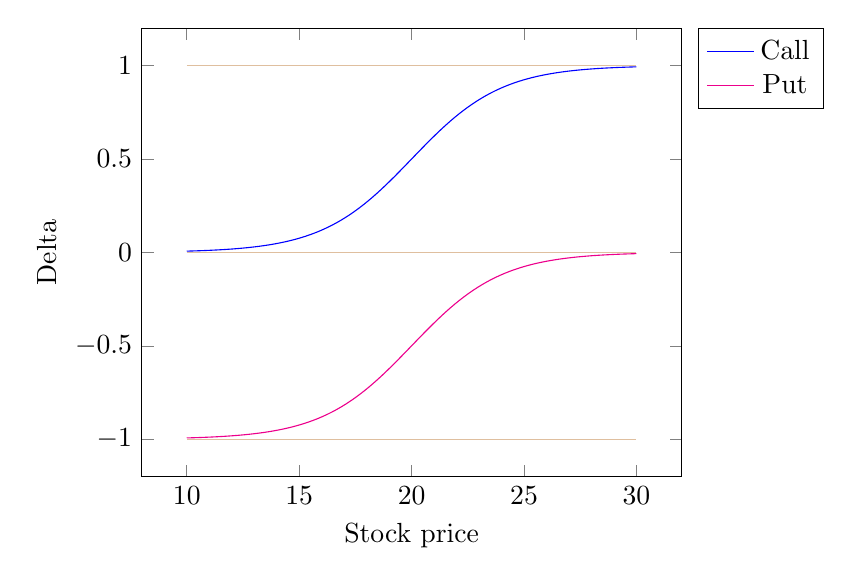
\begin{tikzpicture}
\begin{axis}[domain=10:30, samples=100, xlabel={Stock price}, ylabel={Delta},
legend entries={Call, Put},
legend style={legend pos=outer north east}
]
\addplot[blue]{1/(1+exp(-0.5*(x-20))};
\addplot[magenta]{-1+1/(1+exp(-0.5*(x-20))};
\addplot[brown, opacity=0.5]{0};
\addplot[brown, opacity=0.5]{1};
\addplot[brown, opacity=0.5]{-1};
\end{axis}
\end{tikzpicture}
\end{center}

\item \emph{Property 3: Delta is an increasing function of \(S_0\), with the
most rapid increase occurring near strike price especially for short-lived
options.}

\begin{itemize}
\item \emph{(increasing in \(S_0\))} As \(S_0\) \faIcon{arrow-up}, the call
(put) is more (less) likely to expire in-the-money, thus being more (less)
sensitive to stock price changes. Hence, the call (put) delta becomes more
positive (less negative).

\item \emph{(steep increase near strike price, especially for short-lived
options)} As \(S_0\) increases past the strike price \(K\), the call (put) is
much more (less) likely to expire in-the-money, especially for short-lived ones
as there is not much room for further movements in stock prices for them.

\item \emph{(delta of deep in-the-money option is close to 1 in absolute
value)} We can observe that \(\Delta_0^C\approx 1\) for very high \(S_0\) and
\(\Delta_0^{P}\approx -1\) for very low \(S_0\), meaning that a deep
in-the-money call/put is extremely sensitive to stock price changes --- its
price moves in almost the same magnitude as the stock price!

This is because a deep in-the-money call/put would almost surely expire in the
money, so an unit increase in \(S_0\) would lead to almost an unit increase
(decrease) in the call (put) price.

\item \emph{(delta of deep out-of-the-money option is close to 0)} We can
observe that \(\Delta_0^C\approx 0\) for very low \(S_0\) and
\(\Delta_0^{P}\approx 0\) for very high \(S_0\), meaning that a deep
out-of-the-money has almost no sensitivity to stock price changes. This is
because a deep out-of-the-money call/put would almost surely expire worthless,
so changes in \(S_0\) would hardly lead to any change in the call/put price
(which would be very close to 0 as the call/put is almost a ``trash''
\faIcon{trash-alt}).

\begin{center}
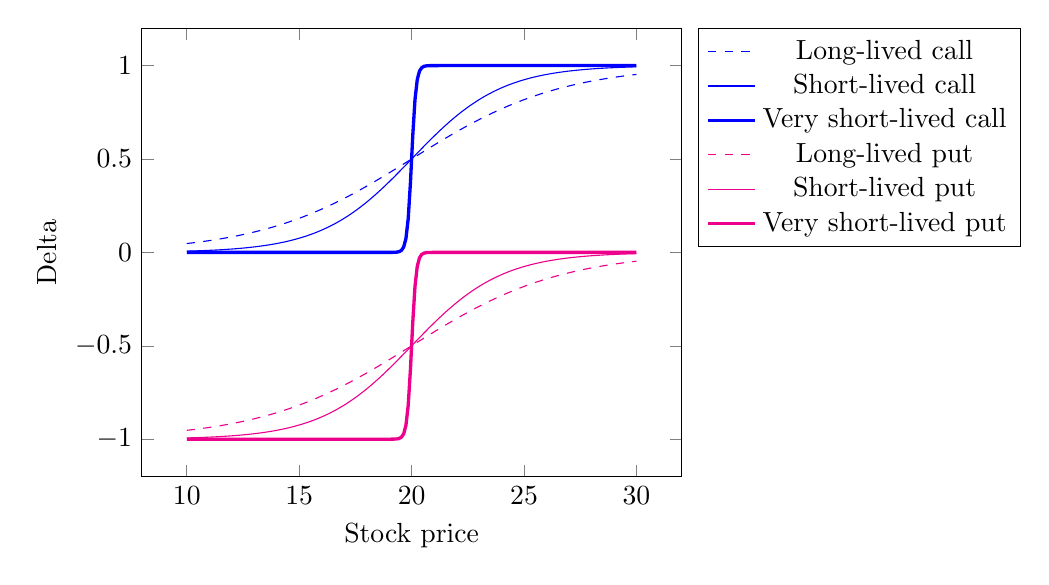
\begin{tikzpicture}
\begin{axis}[domain=10:30, samples=200, xlabel={Stock price}, ylabel={Delta},
legend entries={Long-lived call, Short-lived call, Very short-lived call,
Long-lived put, Short-lived put, Very short-lived put},
legend style={legend pos=outer north east}
]
\addplot[blue, dashed]{1/(1+exp(-0.3*(x-20))};
\addplot[blue]{1/(1+exp(-0.5*(x-20))};
\addplot[blue, very thick]{1/(1+exp(-10*(x-20))};
\addplot[magenta, dashed]{-1+1/(1+exp(-0.3*(x-20))};
\addplot[magenta]{-1+1/(1+exp(-0.5*(x-20))};
\addplot[magenta, very thick]{-1+1/(1+exp(-10*(x-20))};
\end{axis}
\end{tikzpicture}
\end{center}
\end{itemize}
\item \emph{Property 4: Delta gets larger in absolute value as \(T\) increases
for deep out-of-the-money (in-the-money) option (with \(S_0\) fixed).} As a
deep out-of-the-money (in-the-money) option has a longer time to live, there is
a larger room for further movements in stock prices, thus it has a higher
chance to eventually expire in-the-money (out-of-the-money), hence being more
(less) sensitive to the stock price changes.
\begin{center}
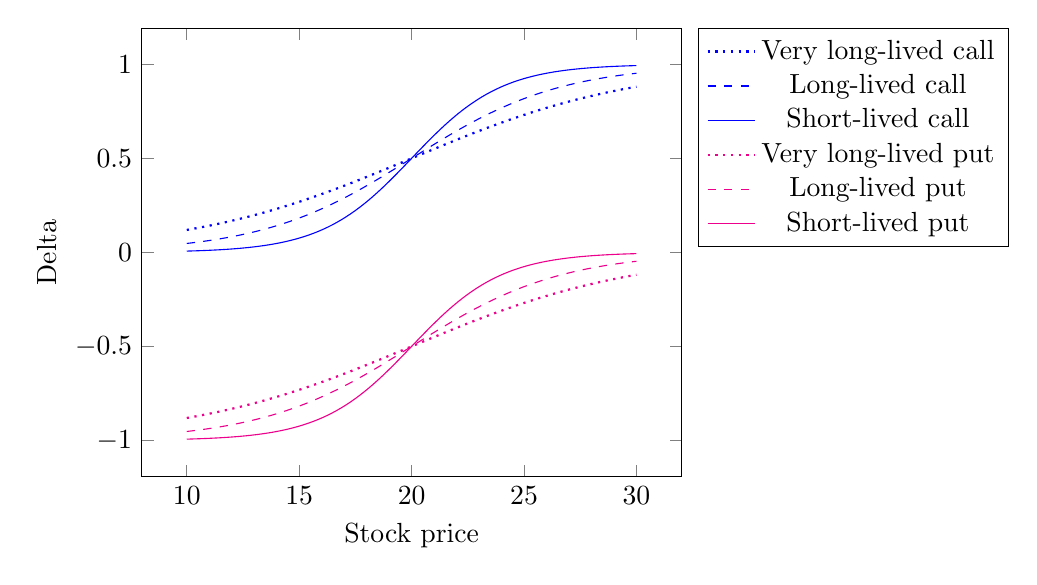
\begin{tikzpicture}
\begin{axis}[domain=10:30, samples=100, xlabel={Stock price}, ylabel={Delta},
legend entries={Very long-lived call, Long-lived call, Short-lived call, Very long-lived put, Long-lived put, Short-lived put},
legend style={legend pos=outer north east}
]
\addplot[blue, thick, dotted]{1/(1+exp(-0.2*(x-20))};
\addplot[blue, dashed]{1/(1+exp(-0.3*(x-20))};
\addplot[blue]{1/(1+exp(-0.5*(x-20))};
\addplot[magenta, thick, dotted]{-1+1/(1+exp(-0.2*(x-20))};
\addplot[magenta, dashed]{-1+1/(1+exp(-0.3*(x-20))};
\addplot[magenta]{-1+1/(1+exp(-0.5*(x-20))};
\end{axis}
\end{tikzpicture}
\end{center}
\end{enumerate}
\subsection{Gamma}
\begin{enumerate}
\item From the graphs for the delta in \Cref{subsect:delta}, we observe that
delta can vary drastically as \(S_0\) changes, so we would like to also study
the sensitivity of delta in response to stock price changes (sensitivity of
sensitivity measures!). This can be done by using gamma.

The \defn{gamma} of an option is the partial derivative of the option delta
with respect to the current price of the underlying asset, i.e., the
second partial derivative of the option price with respect to the current asset
price:
\[
\Gamma_0=\pdv{\Delta_0}{S_0}=\pdv[2]{V_0}{S_0}.
\]
Gamma can be interpreted as (i) a measure of the sensitivity of the delta in
response to asset price changes, or (ii) a measure of the convexity of the
option price as a function of \(S_0\). For the purpose of understanding the
qualitative properties, the interpretation (i) is usually more helpful.

\item \label{it:call-gamma-fmla} To answer \labelcref{it:cpt-greek} for option
gamma, we derive a closed-form formula for the gamma of a European call. By
\labelcref{it:call-delta-fmla} we have \(\Delta_0^C=e^{-\delta T}\Phi(d_1)\).
Then, using chain rule, partially differentiating both sides with respect to
\(S_0\) gives
\[
\Gamma_0^C={\pdv{}{S_0}}[e^{-\delta T}\Phi(d_1)]=e^{-\delta T}\phi(d_1)\pdv{d_1}{S_0}
=\boxed{\frac{e^{-\delta T}\phi(d_1)}{S_0\sigma\sqrt{T}}}.
\]

\item \label{it:call-put-gamma-relate} Next, we will answer
\labelcref{it:call-put-greek}, by partially differentiating the relation
\(\Delta_0^P=\Delta_0^C-e^{-\delta T}\) from
\labelcref{it:call-put-delta-relate}, with respect to \(S_0\):
\[
\pdv{\Delta_0^P}{S_0}=\pdv{\Delta_0^C}{S_0}-\underbrace{\pdv{e^{-\delta T}}{S_0}}_{0}
\implies \Gamma^P_0=\Gamma^C_0,
\]
meaning that the gamma of call and put that are otherwise identical are always
the same. Consequently, when answering \labelcref{it:greek-qual} in the
following, it suffices to focus on call gamma, without loss of generality.

\item \emph{Property 1: Gamma is always positive.} This is because the delta is
a strictly increasing function of \(S_0\), as we have seen in
\Cref{subsect:delta}.

\begin{center}
\begin{tikzpicture}
\begin{axis}[domain=10:30, samples=200, xlabel={Stock price}, ylabel={Gamma},
yticklabel style={/pgf/number format/fixed}, scaled y ticks=false,
legend entries={Call},
legend style={legend pos=outer north east}
]
\addplot[blue]{0.00000001*(x-4)^(10)*exp(-0.8*(x-4))};
\end{axis}
\end{tikzpicture}
\end{center}

\item \emph{Property 2: Gamma is almost zero for deep
in-the-money/out-of-the-money option.} When the call is deep in-the-money
(out-of-the-money), the delta is extremely close to \(1\) (\(0\)) and hardly
response to any change in stock price.
\begin{center}
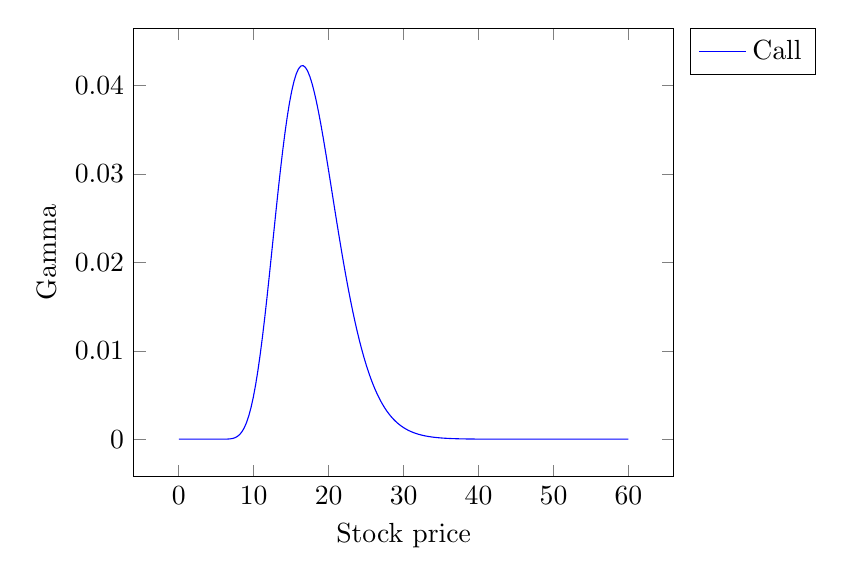
\begin{tikzpicture}
\begin{axis}[domain=0:60, samples=200, xlabel={Stock price}, ylabel={Gamma},
yticklabel style={/pgf/number format/fixed}, scaled y ticks=false,
legend entries={Call},
legend style={legend pos=outer north east}
]
\addplot[blue]{(x>=4)*0.00000001*(x-4)^(10)*exp(-0.8*(x-4))};
\end{axis}
\end{tikzpicture}
\end{center}

\item \emph{Property 3: Gamma is very large when the stock price is near the
strike price, especially for short-lived options.} This follows from the
property of delta that it rises most rapidly near the strike price especially
for short-lived options, thus the rate of change of delta is very large around
that region, hence a larger gamma.
\begin{center}
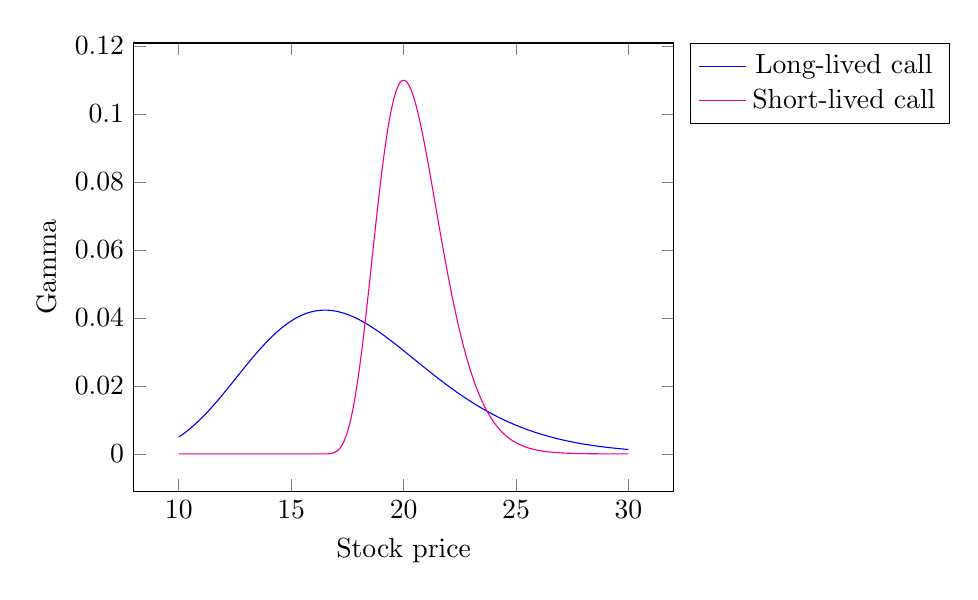
\begin{tikzpicture}
\begin{axis}[domain=10:30, samples=200, xlabel={Stock price}, ylabel={Gamma},
yticklabel style={/pgf/number format/fixed}, scaled y ticks=false,
legend entries={Long-lived call, Short-lived call},
legend style={legend pos=outer north east}
]
\addplot[blue]{0.00000001*(x-4)^(10)*exp(-0.8*(x-4))};
\addplot[magenta]{(x>=16)*0.005*(x-16)^(8)*exp(-2*(x-16))};
\end{axis}
\end{tikzpicture}
\end{center}
\end{enumerate}
\subsection{Theta}
\begin{enumerate}
\item The next and final Greek to be discussed here is related to the impact of
\emph{passage of time} on the option price. As passage of time is involved, we
need to analyze the option prices dynamically instead of just focusing on the
time-0 price.

Consider a \(T\)-year European option. The time-\(t\) price of the option
(\(0\le t\le T\)), denoted by \(V_t\), is based on the time-\(t\) underlying
asset price \(S_t\) and the remaining time to expiration \(T-t\).

The (time-\(t\)) \defn{theta} is the partial derivative of the time-\(t\)
option price with respect to the current time \(t\) (here we treat time \(t\)
as ``now''):
\[
\Theta_t=\pdv{V_t}{t}.
\]
The theta \(\Theta_t\) can be interpreted as the approximated change in the
option price \(V_t\) when the remaining time to expiration \(T-t\)
\emph{decreases} by 1 year (i.e., 1 year has ``passed''). Treating 1 day to be
\(1/365\) years, the approximated change after the ``passage'' of 1 day can be
obtained by \(\Theta_t\times (1/365)\).

\item \label{it:call-theta-fmla} We first answer \labelcref{it:cpt-greek} for
theta. It turns out that theta has a rather complicated closed-form formula.
Consider a European call and its time-\(t\) Black-Scholes call price
\[
C_t=\bs{S_t,\delta}{K,r}{\sigma,T-t}=S_te^{-\delta(T-t)}\Phi(d_1)-Ke^{-r(T-t)}\Phi(d_2)
\]
where \(\displaystyle
d_1=\frac{\ln(S_t/K)+(r-\delta+\sigma^2/2)(T-t)}{\sigma\sqrt{T-t}}\) and
\(d_2=d_1-\sigma\sqrt{T-t}\). Partially differentiating the call price \(C_t\)
with respect to the current time \(t\) while holding all other things
fixed\footnote{In particular, we treat \(S_t\) as a fixed value that does not
change with time \(t\). In other words, after the time changes from \(t\) to
some other time \(t^*\), we still use the time-\(t\) price \(S_t\) (the price
at the original time point).} gives
\begin{align*}
\Theta_t^C&=\vc{\delta S_te^{-\delta(T-t)}\Phi(d_1)}+S_te^{-\delta(T-t)}\phi(d_1)\pdv{d_1}{t}
\vc{-rKe^{-r(T-t)}\Phi(d_2)}-Ke^{-r(T-t)}\phi(d_2)\pdv{d_2}{t} \\
&=\vc{\delta S_te^{-\delta(T-t)}\Phi(d_1)-rKe^{-r(T-t)}\Phi(d_2)}
+S_te^{-\delta(T-t)}\phi(d_1)\pdv{d_1}{t}
-Ke^{-r(T-t)}\phi(d_2)\qty(\pdv{d_1}{t}-\frac{\sigma}{2\sqrt{T-t}}) \\
&=\vc{\delta S_te^{-\delta(T-t)}\Phi(d_1)-rKe^{-r(T-t)}\Phi(d_2)}
+[\underbrace{S_te^{-\delta(T-t)}\phi(d_1)-Ke^{-r(T-t)}\phi(d_2)}_{0}]\pdv{d_1}{t} \\
&\quad-Ke^{-r(T-t)}\phi(d_2)\frac{\sigma}{2\sqrt{T-t}} \\
&=\boxed{\delta S_te^{-\delta(T-t)}\Phi(d_1)-rKe^{-r(T-t)}\Phi(d_2)
-\frac{Ke^{-r(T-t)}\phi(d_2)\sigma}{2\sqrt{T-t}}}.
\end{align*}
where \(S_te^{-\delta(T-t)}\phi(d_1)-Ke^{-r(T-t)}\phi(d_2)=0\) can be shown by
using a similar argument as in the proof for the formula for call delta.

\item \label{it:call-put-theta-relate} After that, we shall answer
\label{it:call-put-greek} for theta. Again we will utilize the put-call parity.
Partially differentiating both sides of the put-call parity
\(C_t-P_t=S_te^{-\delta(T-t)}-Ke^{-r(T-t)}\) with respect to \(t\) gives
\[
\Theta_t^{C}-\Theta_t^{P}=\delta S_te^{-\delta(T-t)}-rKe^{-r(T-t)}.
\]
Rearranging this gives
\begin{align*}
\Theta_t^P&=\boxed{\Theta_t^C -\delta S_te^{-\delta(T-t)}+rKe^{-r(T-t)}} \\
&=\delta S_te^{-\delta(T-t)}\Phi(d_1)-rKe^{-r(T-t)}\Phi(d_2)
-\frac{Ke^{-r(T-t)}\phi(d_2)\sigma}{2\sqrt{T-t}}
-\delta S_te^{-\delta(T-t)}+rKe^{-r(T-t)} \\
&=\boxed{\rc{-}\delta S_te^{-\delta(T-t)}\Phi(\rc{-}d_1)\rc{+}rKe^{-r(T-t)}\Phi(\rc{-}d_2)
-\frac{Ke^{-r(T-t)}\phi(d_2)\sigma}{2\sqrt{T-t}}},
\end{align*}
where \(d_1\) and \(d_2\) are based on the time-\(t\) call price \(C_t\).

\item Lastly, we will deal with the somewhat hard-to-answer question:
\labelcref{it:greek-qual} for theta. As hinted by the complicated formulas for
call and put thetas, one can expect that the qualitative properties of theta
are rather complex and the explanations would be quite intricate.

The complex behaviour of theta can be explained through analyzing the following
opposing forces:
\begin{enumerate}[label={F\arabic*}]
\item \label{it:less-uncertainty} \emph{\(t\uparrow\implies \text{less
uncertainty ahead}\implies V_t\downarrow\).}

The option price increases as there is more
uncertainty ahead, due to the \emph{asymmetric} option payoffs. For a call
(put) option:
\begin{itemize}
\item If the stock price falls below (rises above) the strike price, the payoff
would be zero, no matter how far the stock price is away from the strike price.
\item On the other hand, if the stock price rises above (falls below) the
strike price, for every unit increase in the difference, the call payoff would
increase by the same amount.
\end{itemize}
Hence, as the stock price fluctuates in a larger magnitude, the option holder
would benefit more from the upside and would \emph{not} lose more from the
downside, making the option more valuable.

\item\label{it:receive-sooner} \begin{itemize}
\item \emph{call: \(t\uparrow \implies \text{receive underlying asset sooner}
\implies V_t\uparrow\).}
\item \emph{put: \(t\uparrow \implies \text{receive strike price sooner}
\implies V_t\uparrow\).}
\end{itemize}
As the remaining time to expiration reduces, the holder of a call (put), if
exercised, will receive the underlying stock (strike price) and
earn dividends (interest) sooner, making the option more valuable.

\item\label{it:lose-sooner} \begin{itemize}
\item \emph{call: \(t\uparrow \implies \text{lose strike price sooner}
\implies V_t\downarrow\).}
\item \emph{put: \(t\uparrow \implies \text{lose underlying asset sooner}
\implies V_t\downarrow\).}
\end{itemize}
As the remaining time to expiration reduces, the holder of a call (put), if
exercised, will lose the strike price (underlying asset) and lose interest
(dividends) sooner, making the option less valuable.
\end{enumerate}

\item \emph{Property 1: Theta is \underline{mostly} negative.} In view of this,
we say that \underline{most} options suffer from \defn{time decay}. This is
because the force \labelcref{it:less-uncertainty} is dominating for most
options, hence the option price drops as the remaining time to maturity
decreases (all else equal).

\begin{center}
\begin{tikzpicture}
\begin{axis}[domain=10:30, samples=200, xlabel={Stock price}, ylabel={Theta},
yticklabel style={/pgf/number format/fixed}, scaled y ticks=false,
legend entries={Call, Put},
legend style={legend pos=outer north east}
]
\addplot[blue]{-0.00000000002*(x-6)^(14)*exp(-0.8*(x-6))+(x>=27)*1.5*ln(x-26)^2};
\addplot[blue, dashed]{-0.00008*(34-x)^(8)*exp(-0.8*(34-x))+(x<=17)*0.5*ln(18-x)};
\addplot[brown, opacity=0.5]{0};
\end{axis}
\end{tikzpicture}
\end{center}

Yet, in some rare cases, theta can be positive. For this to happen, the force
\labelcref{it:receive-sooner} needs to outweigh the forces
\labelcref{it:less-uncertainty} and \labelcref{it:lose-sooner} combined.
Examples:
\begin{itemize}
\item \emph{deep in-the-money call on a dividend-paying stock:} The time-\(T\)
payoff of such deep-in-the-money call (with very small strike price \(K\)) is
extremely close to \(S_T\), so the call is extremely similar to a prepaid
forward on the stock.  Hence, its time-\(t\) price is \(C_t\approx
S_te^{-\delta(T-t)}\), which is a strictly increasing function of \(t\) when
\(\delta>0\). (\(S_t\) is held constant and does not vary with \(t\).)

\item \emph{deep in-the-money put:} The time-\(T\) payoff of such
deep-in-the-money put (with very large strike price \(K\)) is extremely close
to \(K\), so the put is extremely similar to a zero-coupon bond of \(K\)
maturing at time \(T\).  Hence, its time-\(t\) price is \(P_t\approx
Ke^{-r(T-t)}\), which is also a strictly increasing function of \(t\).
\end{itemize}

\item \emph{Property 2: Theta is close to zero for deep out-of-the-money
options, especially for short-lived ones.} This is because deep
out-of-the-money option has a very high chance to expire worthless, thus does
not response much to changes in the remaining time to maturity.

For short-lived options in particular, as there is only a very short time left
for the stock price to change, the option would almost surely expire worthless,
hence there is virtually no sensitivity to changes in the remaining time to
maturity.

\begin{center}
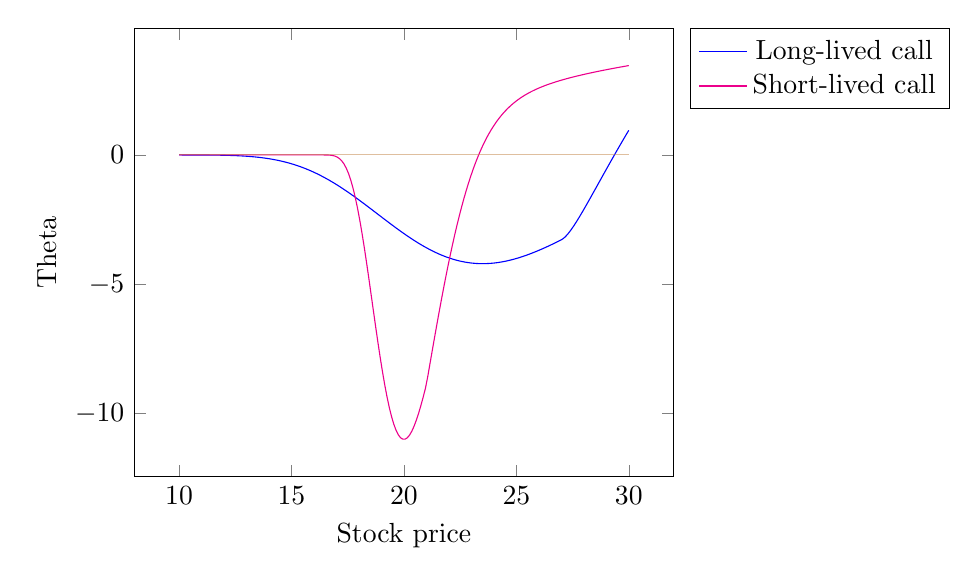
\begin{tikzpicture}
\begin{axis}[domain=10:30, samples=200, xlabel={Stock price}, ylabel={Theta},
yticklabel style={/pgf/number format/fixed}, scaled y ticks=false,
legend entries={Long-lived call, Short-lived call},
legend style={legend pos=outer north east}
]
\addplot[blue]{-0.00000000002*(x-6)^(14)*exp(-0.8*(x-6))+(x>=27)*1.5*ln(x-26)^2};
\addplot[magenta]{-(x>=16)*0.5*(x-16)^(8)*exp(-2*(x-16))+(x>=21)*1.5*ln(x-20)};
\addplot[brown, opacity=0.5]{0};
\end{axis}
\end{tikzpicture}
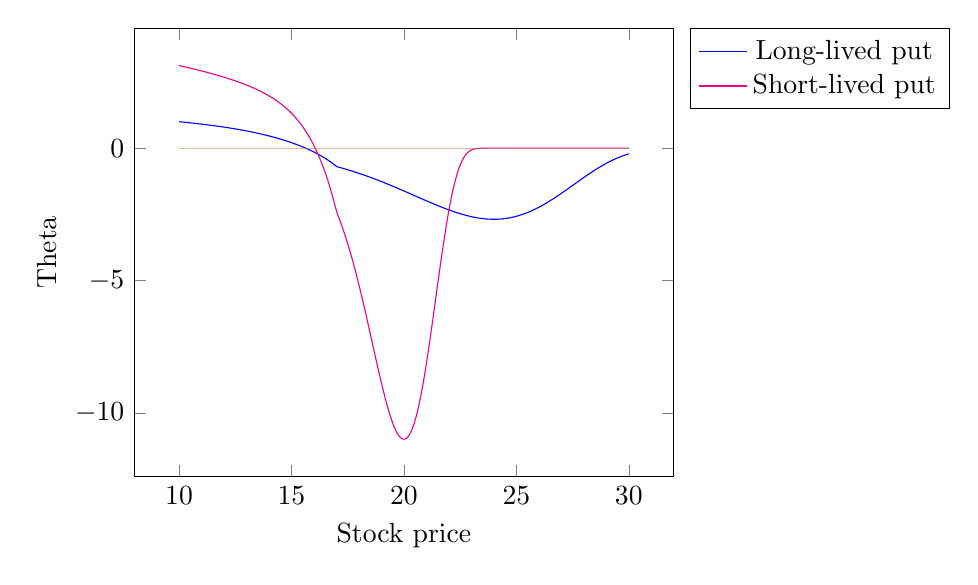
\begin{tikzpicture}
\begin{axis}[domain=10:30, samples=200, xlabel={Stock price}, ylabel={Theta},
yticklabel style={/pgf/number format/fixed}, scaled y ticks=false,
legend entries={Long-lived put, Short-lived put},
legend style={legend pos=outer north east}
]
\addplot[blue]{-0.00008*(34-x)^(8)*exp(-0.8*(34-x))+(x<=17)*0.5*ln(18-x)};
\addplot[magenta]{-(x<=24)*0.5*(24-x)^(8)*exp(-2*(24-x))+(x<=17)*1.5*ln(18-x)};
\addplot[brown, opacity=0.5]{0};
\end{axis}
\end{tikzpicture}
\end{center}

\item \emph{Property 3: Theta is very negative for at-the-money options,
especially for the short-lived ones.} For at-the-money option, changes in stock
price often ``passes through'' the strike price, hence such option gains a lot
from the asymmetry of option payoff. Thus, as the remaining time to maturity
drops, the less uncertainty ahead as suggested in the force
\labelcref{it:less-uncertainty} reduces a huge amount of the option price.

This effect is more significant for short-lived at-the-money options since a
tiny drop in the remaining time to maturity already leads to a relatively large
decrease in the time to maturity.
\begin{center}
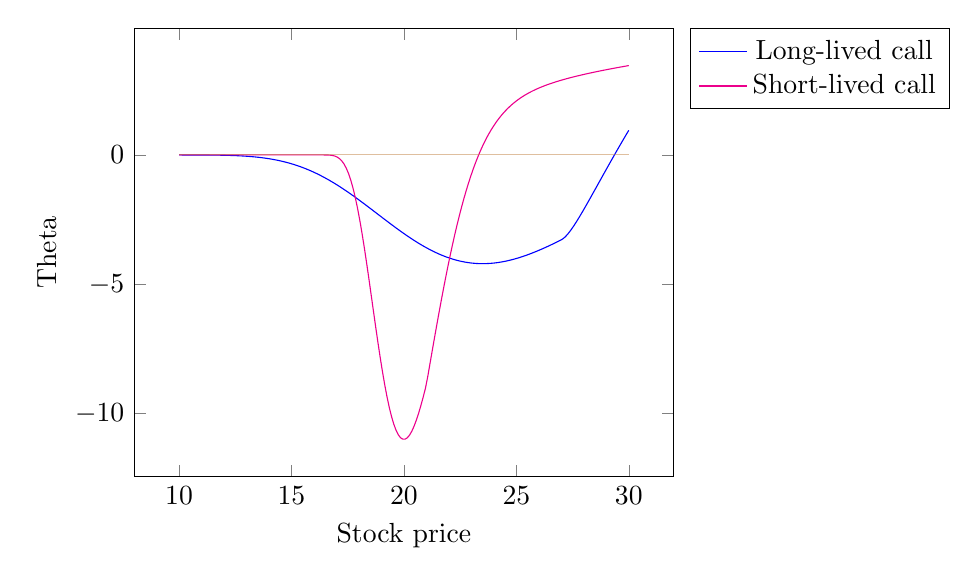
\begin{tikzpicture}
\begin{axis}[domain=10:30, samples=200, xlabel={Stock price}, ylabel={Theta},
yticklabel style={/pgf/number format/fixed}, scaled y ticks=false,
legend entries={Long-lived call, Short-lived call},
legend style={legend pos=outer north east}
]
\addplot[blue]{-0.00000000002*(x-6)^(14)*exp(-0.8*(x-6))+(x>=27)*1.5*ln(x-26)^2};
\addplot[magenta]{-(x>=16)*0.5*(x-16)^(8)*exp(-2*(x-16))+(x>=21)*1.5*ln(x-20)};
\addplot[brown, opacity=0.5]{0};
\end{axis}
\end{tikzpicture}
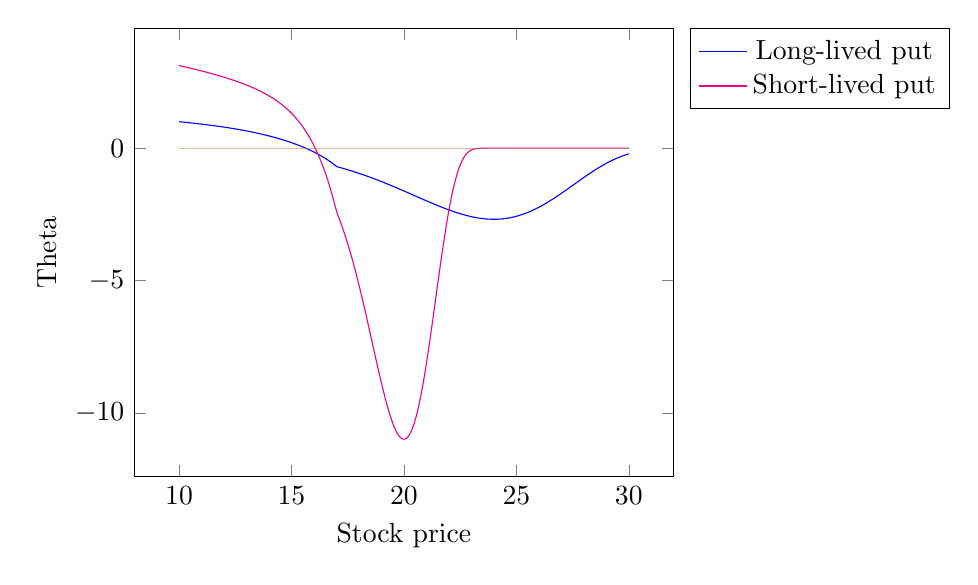
\begin{tikzpicture}
\begin{axis}[domain=10:30, samples=200, xlabel={Stock price}, ylabel={Theta},
yticklabel style={/pgf/number format/fixed}, scaled y ticks=false,
legend entries={Long-lived put, Short-lived put},
legend style={legend pos=outer north east}
]
\addplot[blue]{-0.00008*(34-x)^(8)*exp(-0.8*(34-x))+(x<=17)*0.5*ln(18-x)};
\addplot[magenta]{-(x<=24)*0.5*(24-x)^(8)*exp(-2*(24-x))+(x<=17)*1.5*ln(18-x)};
\addplot[brown, opacity=0.5]{0};
\end{axis}
\end{tikzpicture}
\end{center}
\end{enumerate}
\subsection{Delta-Hedging}
\label{subsect:delta-hedging}
\begin{enumerate}
\item After discussing three option Greeks: delta (\(\Delta\)), gamma
(\(\Gamma\)), theta (\(\Theta\)), we shall discuss how they are useful for
designing and implementing hedging strategies (under Black-Scholes model).
Firstly, we will discuss a simple hedging strategy known as \emph{delta
hedging}.

\item For illustration purpose, in \Cref{sect:bs-model-hedging}, we shall
consider a setting where hedging is critical and we will analyze how different
hedging strategies can protect us. We shall consider the perspective from a
\defn{market-maker}, who is an intermediary or trader that is ready to buy
(sell) derivatives from customers who wish to sell (buy), i.e., a counterparty
to the customers.

For example, assume that a market-maker has \emph{sold} a European call option
on a nondividend-paying stock and has therefore incurred a delta of
\(-\Delta_0^C\) in his portfolio.

\begin{note}
In general, the greek of a \emph{portfolio} is also a partial derivative with
respect to the same input of interest, but the ``option price'' is replaced by
``portfolio value''. For example, in this case, the market-maker's portfolio
consists of \(-1\) unit of call, hence the portfolio delta is
\(\displaystyle \pdv{(-C_0)}{S_0}=-\pdv{C_0}{S_0}=-\Delta_0^C\).
\end{note}

\item Since the market-maker's delta is negative\footnote{Recall that call delta is
always positive.}, he is exposed to \emph{upside} stock price risk, i.e., the
risk that the stock price rises in the future. To be more specific, we consider
the \defn{overnight profit} (i.e., the profit on the next day, or at time
\(1/365\)) of the market-maker.

The overnight profit can be computed by
\[
-C_{1/365}+C_0e^{r/365},
\]
which is the payoff at time \(1/365\) of the following actions performed at
time 0 that result in zero net cash flow at that time:
\begin{enumerate}[label={(\arabic*)}]
\item sell a European call (time-0 CF: \(+C_0\))
\item lend \(C_0\) (time-0 CF: \(-C_0\))
\end{enumerate}
Then, at time \(1/365\), the action (1) results in a payoff of \(-C_{1/365}\)
(from closing out the short call position) and the action (2) results in a
payoff of \(+C_0e^{r/365}\).

\begin{center}
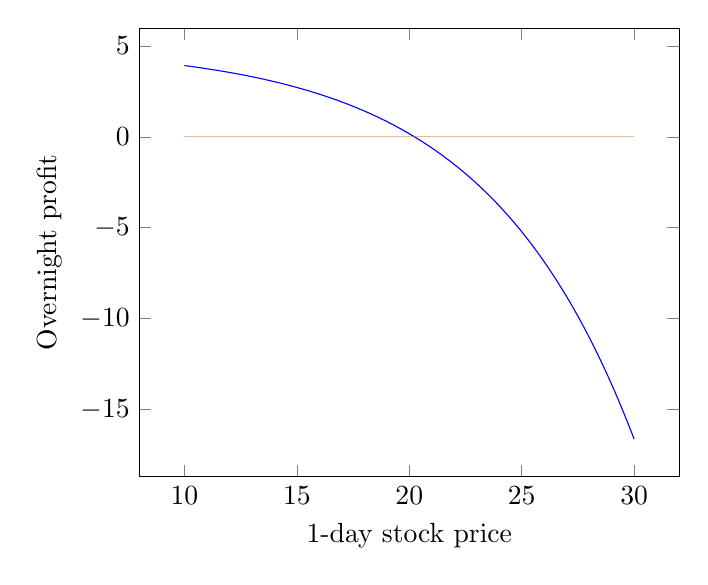
\begin{tikzpicture}
\begin{axis}[domain=10:30, samples=200, xlabel={1-day stock price}, ylabel={Overnight profit},
yticklabel style={/pgf/number format/fixed}, scaled y ticks=false
]
\addplot[blue]{5-exp(-0.15*(9.5-x))};
\addplot[brown, opacity=0.5]{0};
\end{axis}
\end{tikzpicture}
\end{center}

\item We can observe that as \(S_{1/365}\) rises, the overnight profit drops
\emph{indefinitely}! There is no limit on how much the market-maker can lose,
meaning that he can potentially \emph{bankrupt}! In view of this, there is a
desperate need to hedge against this dangerous position \warn{}.

\begin{note}
Sometimes the act of selling a call without owning the underlying asset is
called selling a \defn{naked call} since it is as dangerous as being
``naked''...
\end{note}

\item Market-makers earn profit by buying at the bid price (from customers who
wish to sell immediately) and selling at the ask price (from customers who wish
to buy immediately) to capture by the bid-ask spread, instead of speculating on
the asset prices in the market.

Thus, it is of great interest for market-makers to protect themselves against
the risk arising from their actions, by making the profit graph ``flatter''
(having less potential loss at the cost of having less potential profit from
price movements as well).

\item \label{it:delta-hedging-actions}
A simple way of protection against the risk from selling/writing a call
is \emph{delta-hedging}. To form \defn{delta-hedging}, we perform the following
actions at time 0, in the case of selling call:

\begin{enumerate}[label={(\arabic*)}]
\item sell a European call (time-0 CF: \(+C_0\))
\item buy \(\Delta_0^C\) shares of stock to \emph{delta-hedge} the
market-maker's position (time-0 CF: \(-\Delta_0^CS_0\))
\item borrow \(Ke^{-rT}\Phi(d_2)\) at risk-free interest rate, or investing
\(-Ke^{-rT}\Phi(d_2)\) in a risk-free bond (time-0 CF: \(+Ke^{-rT}\Phi(d_2)\))
\end{enumerate}
Note that the time-0 net cash flow of these actions is
\[
+C_0-\Delta_0^{C}S_0+Ke^{-rT}\Phi(d_2)
=S_0\underbrace{e^{-\delta T}\Phi(d_1)}_{\Delta_0^C}-Ke^{-rT}\Phi(d_2)-\Delta_0^{C}S_0+Ke^{-rT}\Phi(d_2)
=0.
\]

After these actions, the delta of market-maker's portfolio is exactly zero at
time 0, and the portfolio is said to be \defn{delta-neutral}.

\item \label{it:delta-hedging-profit-fmla}
After that, the time-\(t\) profit of a delta-hedged written call is given
by
\[
\underbrace{-C_t}_{(1)}\underbrace{+\Delta_0^CS_t}_{(2)}\underbrace{-B_0e^{rt}}_{(3)}.
\]
\begin{center}
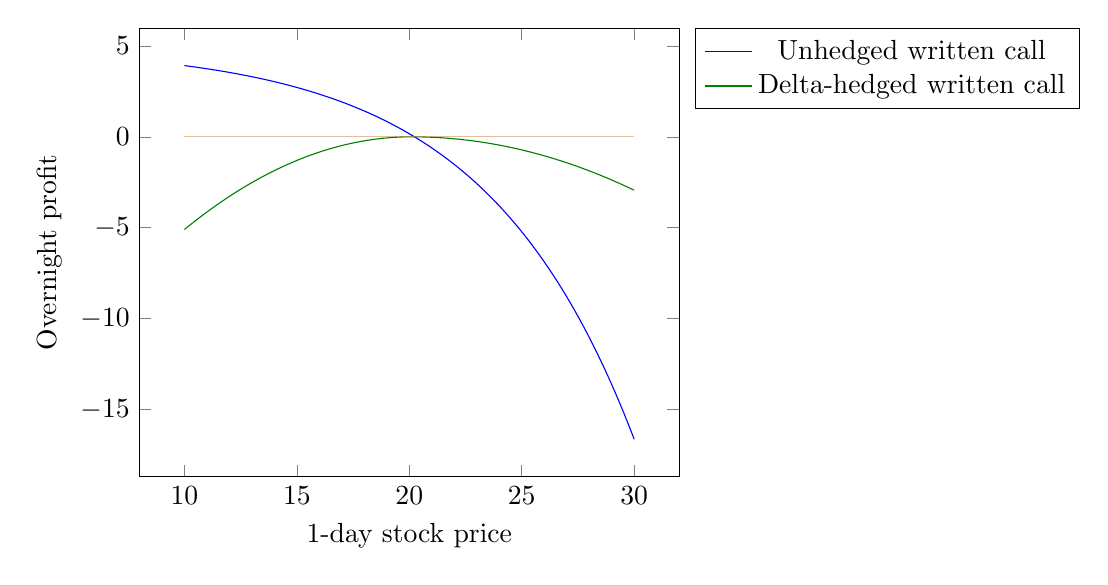
\begin{tikzpicture}
\begin{axis}[domain=10:30, samples=200, xlabel={1-day stock price}, ylabel={Overnight profit},
yticklabel style={/pgf/number format/fixed}, scaled y ticks=false,
legend entries={Unhedged written call, Delta-hedged written call},
legend style={legend pos=outer north east}
]
\addplot[blue]{5-exp(-0.15*(9.5-x))};
\addplot[green!50!black]{-(x<=20.1)*0.05*(x-20.1)^2-(x>20.1)*0.03*(x-20.1)^2};
\addplot[brown, opacity=0.5]{0};
\end{axis}
\end{tikzpicture}
\end{center}

We can observe that after delta-hedging, the market-maker's profit declines at
a more controllable rate as the stock price increases, meaning that the upside
stock price risk drops a lot. In exchange for this protection, the delta-hedged
written call has a negative and decreasing profit when the stock price
decreases, unlike the unhedged written call. Nonetheless, in terms of potential
loss, the delta-hedged written call would be safer.
\end{enumerate}
\subsection{Hedging Multiple Option Greeks}
\label{subsect:hedge-multiple-greeks}
\begin{enumerate}
\item Delta-hedging is by no means perfect. In fact, even the market maker
delta hedges his short call position, there would still be concern on the
upside stock price risk since it is not completely \emph{eliminated}. The
potential loss is still unlimited, and the market-maker still has a potential
to bankrupt (although with a much lower chance).

\item This issue arises since delta-hedging can only form a \emph{local} protection
against the stock price risk. When the 1-day stock price is near the time-0
price, the overnight profit can be ensured to be very close to zero by the
design of delta-hedging.

However, as there is a larger stock price movement and the stock price is quite
far away from the time-0 price, the protection would start to fall apart and
fail to work. This is because the delta varies as the stock price changes. More
specifically, since the market-maker's portfolio has a negative gamma, the
portfolio delta drops as the stock price rises. Particularly, the
market-maker's delta becomes negative again when the stock price rises from the
time-0 price, and thus his portfolio is no longer delta-neutral.

\item Since the root cause for the issue faced by delta-hedging is the negative
gamma, a natural way to tackle this is to not just neutralize delta, but also
neutralize gamma. This motivates us to hedge multiple Greeks (both delta and
gamma in this context).

However, since the gamma of the underlying stock is \(\displaystyle
\pdv[2]{S_0}{S_0}=0\), buying/selling stocks is not helpful for neutralizing
the gamma. We need to also trade other securities in order to neutralize it.

\item \label{it:hedge-multiple-greeks-method}
Consider the general case where we want to hedge a given option position
with respect to \(m\) option Greeks by using \(m\) securities (in addition the
given option). For each \(i=1,\dotsc,m\), we let \(x_i\) be the number of units
to buy for the \(i\)th security. \begin{note}
When \(x_i<0\), it means that we \emph{sell} \(-x_i\) units of the \(i\)th security.
\end{note}

To find the appropriate number of units to buy for each security that can
neutralize all the \(m\) Greeks, we need to solve the following system of \(m\)
linear equations (one for each Greek) for \(x_1,\dotsc,x_m\):
\[
\begin{cases}
\text{Greek 1 of whole portfolio}=0 \\
\text{Greek 2 of whole portfolio}=0 \\
\hspace{2cm}\vdots \\
\text{Greek \(m\) of whole portfolio}=0,
\end{cases}
\]
where the LHS of each equation is a linear combination of \(x_1,\dotsc,x_m\),
depending on the values of Greeks for each security.

\item In our case here, we want to hedge both delta and gamma. Suppose that the
call sold by the market-maker is of 20-strike. Then, we may utilize a 25-strike
call on the same underlying asset to perform the delta-gamma-hedging. Let
\(x_1\) and \(x_2\) be the number of units to buy for the stock and the
25-strike call. Then, the system we need to solve is
\[
\begin{cases}
x_1(1)+x_2\Delta_0^{C, K=25}-\Delta_0^{C, K=20}&=0 \\
x_1(0)+x_2\Gamma_0^{C, K=25}-\Gamma_0^{C, K=20}&=0
\end{cases}
\]
where the superscripts of the Greeks signify the call strike prices.

After performing the delta-gamma-hedging, the overnight profit would look
something like below.

\begin{center}
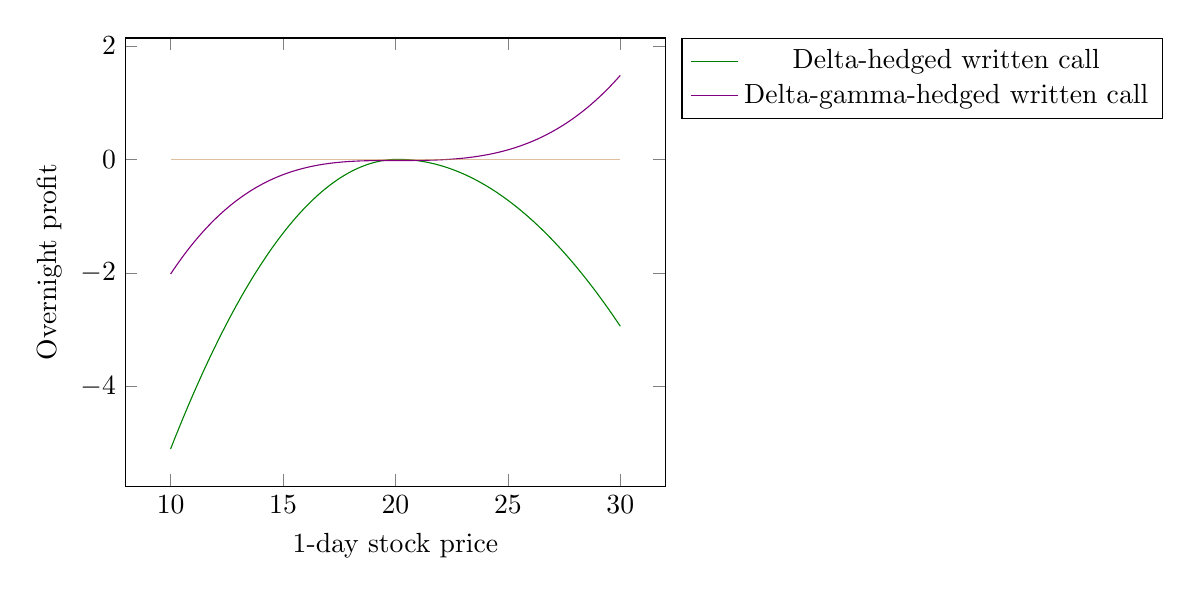
\begin{tikzpicture}
\begin{axis}[domain=10:30, samples=200, xlabel={1-day stock price}, ylabel={Overnight profit},
yticklabel style={/pgf/number format/fixed}, scaled y ticks=false,
legend entries={Delta-hedged written call, Delta-gamma-hedged written call},
legend style={legend pos=outer north east}
]
\addplot[green!50!black]{-(x<=20.1)*0.05*(x-20.1)^2-(x>20.1)*0.03*(x-20.1)^2};
\addplot[violet]{(x<=20)*0.002*(x-20)^3-0.01+(x>20)*0.0015*(x-20)^3-0.01};
\addplot[brown, opacity=0.5]{0};
\end{axis}
\end{tikzpicture}
\end{center}
To inspect the graph more clearly, we zoom in the graph for the part where the
stock price is near 20:
\begin{center}
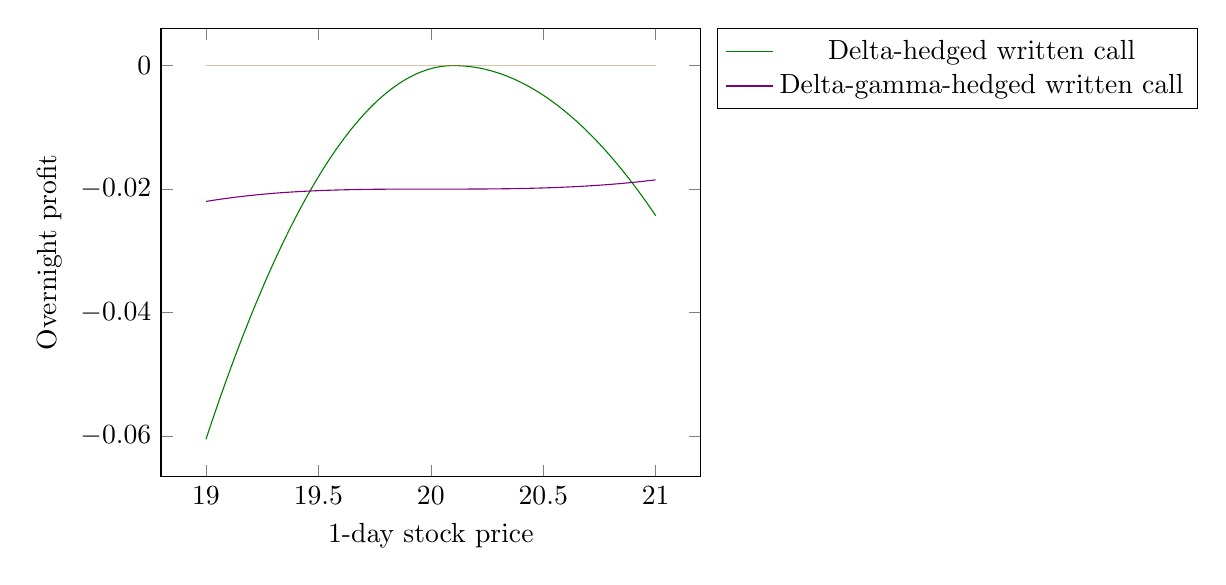
\begin{tikzpicture}
\begin{axis}[domain=19:21, samples=200, xlabel={1-day stock price}, ylabel={Overnight profit},
yticklabel style={/pgf/number format/fixed}, scaled y ticks=false,
legend entries={Delta-hedged written call, Delta-gamma-hedged written call},
legend style={legend pos=outer north east}
]
\addplot[green!50!black]{-(x<=20.1)*0.05*(x-20.1)^2-(x>20.1)*0.03*(x-20.1)^2};
\addplot[violet]{(x<=20)*0.002*(x-20)^3-0.01+(x>20)*0.0015*(x-20)^3-0.01};
\addplot[brown, opacity=0.5]{0};
\end{axis}
\end{tikzpicture}
\end{center}
We can observe that delta-gamma-hedging has a much better performance than
delta-hedging. Not only the upside stock price risk is virtually nonexistent,
the downside stock price risk is also reduced (as the overnight profit when the
stock price drops becomes less negative). In exchange for this improvement,
when the stock price does not move much after 1 day (which is quite likely in
such a short time span), the overnight profit becomes more negative. Still,
delta-gamma-hedging is a much more prudent and effective hedging strategy than
mere delta-hedging.
\end{enumerate}

\subsection{Dynamic Hedging}
\label{subsect:dynamic-hedge-greeks}
\begin{enumerate}
\item Throughout \Cref{subsect:dynamic-hedge-greeks}, we shall assume that the
underlying stock does not pay dividends.

Apart from hedging multiple option Greeks, another possible approach to improve
the effectiveness of delta-hedging is to perform \emph{dynamic hedging},
somewhat like what we do in \Cref{subsect:dynamic-hedging}.

\item Like \Cref{subsect:dynamic-hedging}, here we also need to construct
replicating portfolios dynamically, but we are doing that in the Black-Scholes
model rather than the binomial tree model. \begin{note}
In this context, another name for replicating portfolio is \defn{hedge portfolio}.
\end{note}
Recall from \Cref{subsect:delta-hedging} that to perform delta-hedging of a
written call, we need to do the following actions at time 0 (in addition to
selling the call):
\begin{itemize}
\item \emph{(stock part)} buying \(\Delta_0^C=\Phi(d_1)\) shares of the stock 
\item \emph{(bond part)} investing \(B_0=-Ke^{-rT}\Phi(d_2)\) in a risk-free
bond
\end{itemize}
Note that the number of shares in the stock part is the ``coefficient'' of
\(S_0\) in the Black-Scholes pricing formula, and the value for the bond part
is precisely the other term in that formula. \begin{note}
This is the same in the case of delta-hedging of a written \emph{put}.
\end{note}

Hence, these actions form a portfolio with time-0 price
\[
\Delta_0^CS_0+B_0=S_0\Phi(d_1)-Ke^{-rT}\Phi(d_2)=C_0,
\]
which replicates the value of the call at time 0. However, as time passes, the
call value would change and hence the old portfolio \((\Delta_0^C,B_0)\) is
generally unable to replicate it. We need to adjust the stock and bond parts in
the portfolio, just like \Cref{subsect:dynamic-hedging}.

\item But under the Black-Scholes model, the call price can \emph{vary
continuously}, unlike the case in the binomial tree model. Consequently, as one
may expect, the adjustment needs to take place in a continuous manner to
successfully complete the replication. It turns out that such continuous
rebalancing requires no cost (the portfolio is self-financing). More details
will be discussed in STAT3911.

\item In practice, it is impossible to rebalance continuously. One can only do
so at discrete time points. So here we shall investigate the effect of
rebalancing at some regular intervals, like monthly, weekly, daily, etc.

Since we are only doing rebalancing at discrete time points rather than in a
continuous manner, our dynamic replicating portfolio will neither be able
complete the replication \emph{perfectly} nor be self-financing. The value of
our portfolio will only approximate the option payoff at maturity, and in each
rebalancing nonzero cash flow may arise due to the mismatch between the values
of the hedge portfolio \emph{needed} (the new one) and the replicating
portfolio \emph{available} (the old one ``brought forward''). (In contrast, if
the rebalancing is done continuously, then these two values coincide.)

\item \label{it:dyna-hedge-port-val-need-avail-fmlas}
More specifically, suppose the current time is \(t\) and we have set up
the hedge portfolio \((\Delta_t,B_t)\) for an European call/put, and the next
rebalancing time is \(t+h\).
\begin{itemize}
\item \emph{value needed at time \(t+h\):} The proper hedge portfolio needed at
time \(t+h\) becomes \((\Delta_{t+h},B_{t+h})\), and the total cost of setting
such portfolio up is the time-\(t+h\) option price:
\[
V_{t+h}=\boxed{\Delta_{t+h}S_{t+h}+B_{t+h}}.
\]
\item \emph{value available at time \(t+h\):} The value of the old hedge
portfolio created at time \(t\) \emph{brought forward} to time \(t+h\) is
\[
V_{t+h}^{\mathrm{bf}}=\boxed{\Delta_tS_{t+h}+B_te^{rh}}.
\]
Here, ``brought forward'' means that we hold the old hedge portfolio from time
\(t\) to \(t+h\). When the time reaches \(t+h\), the new stock price is
\(S_{t+h}\) (while the number of shares owned remains the same due to the
absence of dividends) and the value of risk-free investment grows to
\(B_te^{rh}\) (at the risk-free interest rate \(r\)).
\end{itemize}

\item \label{it:dyna-hedge-ncf-fmla}
In general, \(V_{t+h}\) and \(V_{t+h}^{\mathrm{bf}}\) are different, and the
difference \(V_{t+h}-V_{t+h}^{\mathrm{bf}}\) is the additional cash flow (``net
cash flow'') required to be injected, for rebalancing at time \(t+h\) (this is
also known as \defn{rebalancing cost}):
\[
\text{Net cash flow}_{t+h}=V_{t+h}-V_{t+h}^{\mathrm{bf}}.
\]
If \(\text{Net cash flow}_{t+h}>0\), then extra fund needs to be injected to
update the hedge portfolio \faIcon[regular]{frown}. On the other hand, if \(\text{Net
cash flow}_{t+h}<0\), then some amount of money can be extracted during the
rebalancing \faIcon[regular]{smile}.

\item To compute all the net cash flows involved in the time points
\(0,h,2h,\dotsc,T\), we can use the following table and the formulas above
repetitively:
\begin{center}
\begin{tabular}{cc|ccc|cc}
\toprule
Time \(t\)&\(S_t\)&Stock part& Bond Part&Total&Old hedge brought forward \(V_t^{\mathrm{bf}}\)&Net cash flow\\
\midrule
\(0\)&\(S_0\)&\(\Delta_0\)&\(B_0\)&\(V_0\)&\(0\)&\(V_0\) \\
\(h\)&\(S_h\)&\(\Delta_h\)&\(B_h\)&\(V_h\)&\(\Delta_0 S_h+B_0e^{rh}\)&\(V_h-V_h^{\mathrm{bf}}=?\)\\
\vdots&\vdots&\vdots&\vdots&\vdots&\vdots&\vdots \\
\(kh\)&\(S_{kh}\)&\(\Delta_{kh}\)&\(B_{kh}\)&\(V_{kh}\)&\(\Delta_{(k-1)h}S_{kh}+B_{(k-1)h}e^{rh}\)&\(V_{kh}-V_{kh}^{\mathrm{bf}}=\)?\\
\vdots&\vdots&\vdots&\vdots&\vdots&\vdots&\vdots \\
\(T\)&\(S_{T}\)&\(\Delta_{T}\)&\(B_{T}\)&\(V_{T}\)&\(\Delta_{T-h}S_T+B_{T-h}e^{rh}\)&\(V_{T}-V_{T}^{\mathrm{bf}}=\)?\\
\bottomrule
\end{tabular}
\end{center}
\begin{note}
\(V_T\) equals the payoff the option at maturity.
\end{note}
\end{enumerate}

